\documentclass[11pt,a4paper]{article}

%%%%%%%%%%%%%%%%%%%%%%%%%%%%%%%%%%
% Encoding and language
\usepackage[utf8]{inputenc}
\usepackage[T1]{fontenc}
\usepackage[english]{babel}
\selectlanguage{English}

%%%%%%%%%%%%%%%%%%%%%%%%%%%%%%%%%%
% General packages
\usepackage{verbatim}
\usepackage[all]{xy}
\usepackage{float}
\usepackage{amsmath}
\usepackage{array}
\usepackage{listings}
\usepackage{xcolor}
\usepackage{setspace}
\usepackage{booktabs}
\usepackage{graphicx}
\usepackage{url}
\usepackage{lmodern}
\interfootnotelinepenalty=10000

%%%%%%%%%%%%%%%%%%%%%%%%%%%%%%%%%%
% Page layout
\usepackage{geometry}
\geometry{margin=2.5cm}

%%%%%%%%%%%%%%%%%%%%%%%%%%%%%%%%%%
% Hyperlinks
\usepackage[
    colorlinks=true,
    urlcolor=blue!50!black,
    linkcolor=black,
    citecolor=black
]{hyperref}

%%%%%%%%%%%%%%%%%%%%%%%%%%%%%%%%%%
% Bibliography
\usepackage[round]{natbib}

%%%%%%%%%%%%%%%%%%%%%%%%%%%%%%%%%%
% Fancy headers (ALL pages incl. title page)
\usepackage{fancyhdr}
\pagestyle{fancy}

\fancyhf{} % clear header/footer

\fancyhead[L]{zpn710, fps618, kvb125, xnc401 - everyone contributed equally}
\fancyhead[R]{February 2026}
\fancyfoot[C]{\thepage}

\renewcommand{\headrulewidth}{0.4pt}
\renewcommand{\footrulewidth}{0pt}

% IMPORTANT: make 'plain' style match 'fancy'
\fancypagestyle{plain}{
    \fancyhf{}
    \fancyhead[L]{zpn710, fps618, kvb125, xnc401 - everyone contributed equally}
    \fancyhead[R]{February 2026}
    \fancyfoot[C]{\thepage}
    \renewcommand{\headrulewidth}{0.4pt}
}

%%%%%%%%%%%%%%%%%%%%%%%%%%%%%%%%%%
% Listings styles
\lstdefinestyle{CStyle}{
    language=C,
    basicstyle=\small\ttfamily,
    keywordstyle=\color{blue},
    commentstyle=\color{green!40!black},
    stringstyle=\color{orange},
    numbers=left,
    numberstyle=\tiny,
    stepnumber=1,
    numbersep=5pt,
    backgroundcolor=\color{gray!5},
    frame=single,
    rulecolor=\color{black!30},
    captionpos=b,
    breaklines=true,
    breakatwhitespace=true,
    tabsize=4,
    showspaces=false,
    showstringspaces=false,
}

\definecolor{bluekeywords}{rgb}{0.13,0.13,1}
\definecolor{greencomments}{rgb}{0,0.5,0}
\definecolor{turqusnumbers}{rgb}{0.17,0.57,0.69}
\definecolor{redstrings}{rgb}{0.5,0,0}

\lstdefinelanguage{FSharp}{
    morekeywords={let,new,match,with,rec,open,module,namespace,type,of,member,and,for,in,do,begin,end,fun,function,try,mutable,if,then,else},
    keywordstyle=\color{bluekeywords},
    sensitive=false,
    morecomment=[l][\color{greencomments}]{///},
    morecomment=[l][\color{greencomments}]{//},
    morecomment=[s][\color{greencomments}]{{(*}{*)}},
    morestring=[b]",
    stringstyle=\color{redstrings}
}

%%%%%%%%%%%%%%%%%%%%%%%%%%%%%%%%%%
% Matrix spacing fix
\makeatletter
\renewcommand*\env@matrix[1][*\c@MaxMatrixCols c]{%
  \hskip -\arraycolsep
  \let\@ifnextchar\new@ifnextchar
  \array{#1}}
\makeatother

%%%%%%%%%%%%%%%%%%%%%%%%%%%%%%%%%%
% Graphics paths
\graphicspath{{figures/}{anotherFigureDirectory/}}

%%%%%%%%%%%%%%%%%%%%%%%%%%%%%%%%%%
% Title (no author/date under title)
\title{\LARGE \textbf{Handin 5 Numerical Optimization}}
\date{}

\makeatletter
\def\@maketitle{%
  \newpage
  \vskip 0em % ← space above title (adjust if you want)
  \begin{center}%
    {\LARGE \bfseries \@title \par}%
    \vskip 0.2em % ← space below title (THIS controls the gap)
  \end{center}%
}
\makeatother

%%%%%%%%%%%%%%%%%%%%%%%%%%%%%%%%%%
\begin{document}

\maketitle


\section{Introduction}

In this assignment, we study optimisation with linear equality constraints. 
We first prove a characterisation of the tangent cone, which identifies the feasible directions as the null space of the constraint gradients. Based on this geometric insight, we implement constrained Newton's method and Steepest Descent using projections onto the feasible subspace, and evaluate their performance numerically for varying numbers of constraints.

\section{Proof of Lemma 7}

We consider an $n$-dimensional optimisation problem with $m$ linear equality constraints
\[
c_i(x)=a_i^\top x + b_i = 0,\qquad i=1,\dots,m,\quad \|a_i\|>0
\]
and no inequality constraints. Then the tangent cone at a feasible point $x \in C$ is given by
\[
T_C(x)=\{\,p\in\mathbb{R}^n \mid a_i^\top p = 0,\ i=1,\dots,m\,\}
\]
We use the definition of the tangent cone from the course notes:  
A vector $p \in \mathbb{R}^n$ belongs to $T_C(x)$ if there exists $u>0$ and a curve 
$z:[0,u)\to C$ that is differentiable at $\alpha=0$, with
\[
z(0)=x, \qquad z'(0)=p
\]
We prove the statement by showing both inclusions.

\paragraph{($\subseteq$)} 
We first assume that $p \in T_C(x)$.  
Then there exists a differentiable curve $z(\alpha)\in C$ with $z(0)=x$ and $z'(0)=p$.  
Since $z(\alpha)$ is feasible for all sufficiently small $\alpha$, the constraints satisfy
\[
c_i(z(\alpha)) = a_i^\top z(\alpha) + b_i = 0,
\qquad \text{for all } \alpha \text{ and all } i
\]
We differentiate this identity with respect to $\alpha$ at $\alpha=0$. Because $c_i$ is linear, we obtain
\[
0 
= \frac{d}{d\alpha} c_i(z(\alpha))\Big|_{\alpha=0}
= a_i^\top z'(0)
= a_i^\top p
\]
Hence $a_i^\top p=0$ for all $i=1,\dots,m$, which shows
\[
p \in \{\,p \in \mathbb{R}^n \mid a_i^\top p = 0 \,\}
\]

\paragraph{($\supseteq$)} 
Conversely, we assume that $p \in \mathbb{R}^n$ satisfies $a_i^\top p = 0$ for all $i$. We consider the curve
\[
z(\alpha) = x + \alpha p,
\qquad \alpha \ge 0
\]
Clearly, $z(0)=x$ and $z'(0)=p$. Moreover, for each constraint we compute
\[
c_i(z(\alpha))
= a_i^\top (x+\alpha p) + b_i
= (a_i^\top x + b_i) + \alpha a_i^\top p
\]
Since $x$ is feasible, $a_i^\top x + b_i = 0$, and by assumption $a_i^\top p=0$.  
Therefore $c_i(z(\alpha))=0$ for all $\alpha$, so $z(\alpha)\in C$.
\newline
\newline
By the definition of the tangent cone, this implies $p \in T_C(x)$.Since both inclusions hold, we conclude
\[
T_C(x)=\{\,p\in\mathbb{R}^n \mid a_i^\top p = 0,\ i=1,\dots,m\,\}
\]

\section{Numerical Experiments with Linear Equality Constraints}

\subsection{Correctness of Implementation}
Both algorithms were implemented directly from the pseudocode (Algorithms 10 and 11).
Since Newton's method and steepest descent have been implemented and validated in
previous assignments, our primary concern here was ensuring that the iterates remain
within the feasible set, i.e., that $Ax_k + b = 0$ is satisfied at every step.
To verify this, we computed $\|Ax_k + b\|$ for every iterate across all runs, all
functions, and all values of $m$ both in the case where the unconstrained minimum
$x^*$ is feasible and where it is not. The observed violations ranged from
$4.4 \times 10^{-14}$ to $4.2 \times 10^{-12}$, which is consistent with
floating-point rounding errors and confirms that no iterate ever left the feasible set.
Combined with the convergence results shown in the plots below, where the projected
gradient norm $\|M \nabla f(x_k)\|$ reliably decreases to the tolerance
$\varepsilon = 10^{-6}$, we are confident that the implementation is correct.

\subsection{Stopping criteria}
We compute
\[
M = I - A^\top(AA^\top)^{-1}A
\]
which is the orthogonal projector onto the tangent space (the feasible
directions). We use the stopping criterion
\[
\|M \nabla f(x_k)\| \le \varepsilon
\]
By Theorem~8 and Lemma~9, this corresponds to approximately satisfying
the first-order necessary optimality condition for the equality-constrained
problem, i.e. there exists a multiplier $\lambda$ such that
\[
\nabla f(x_k) + A^\top \lambda \approx 0
\]

\subsection{Results of Performance}

\begin{figure}[H]
    \centering
    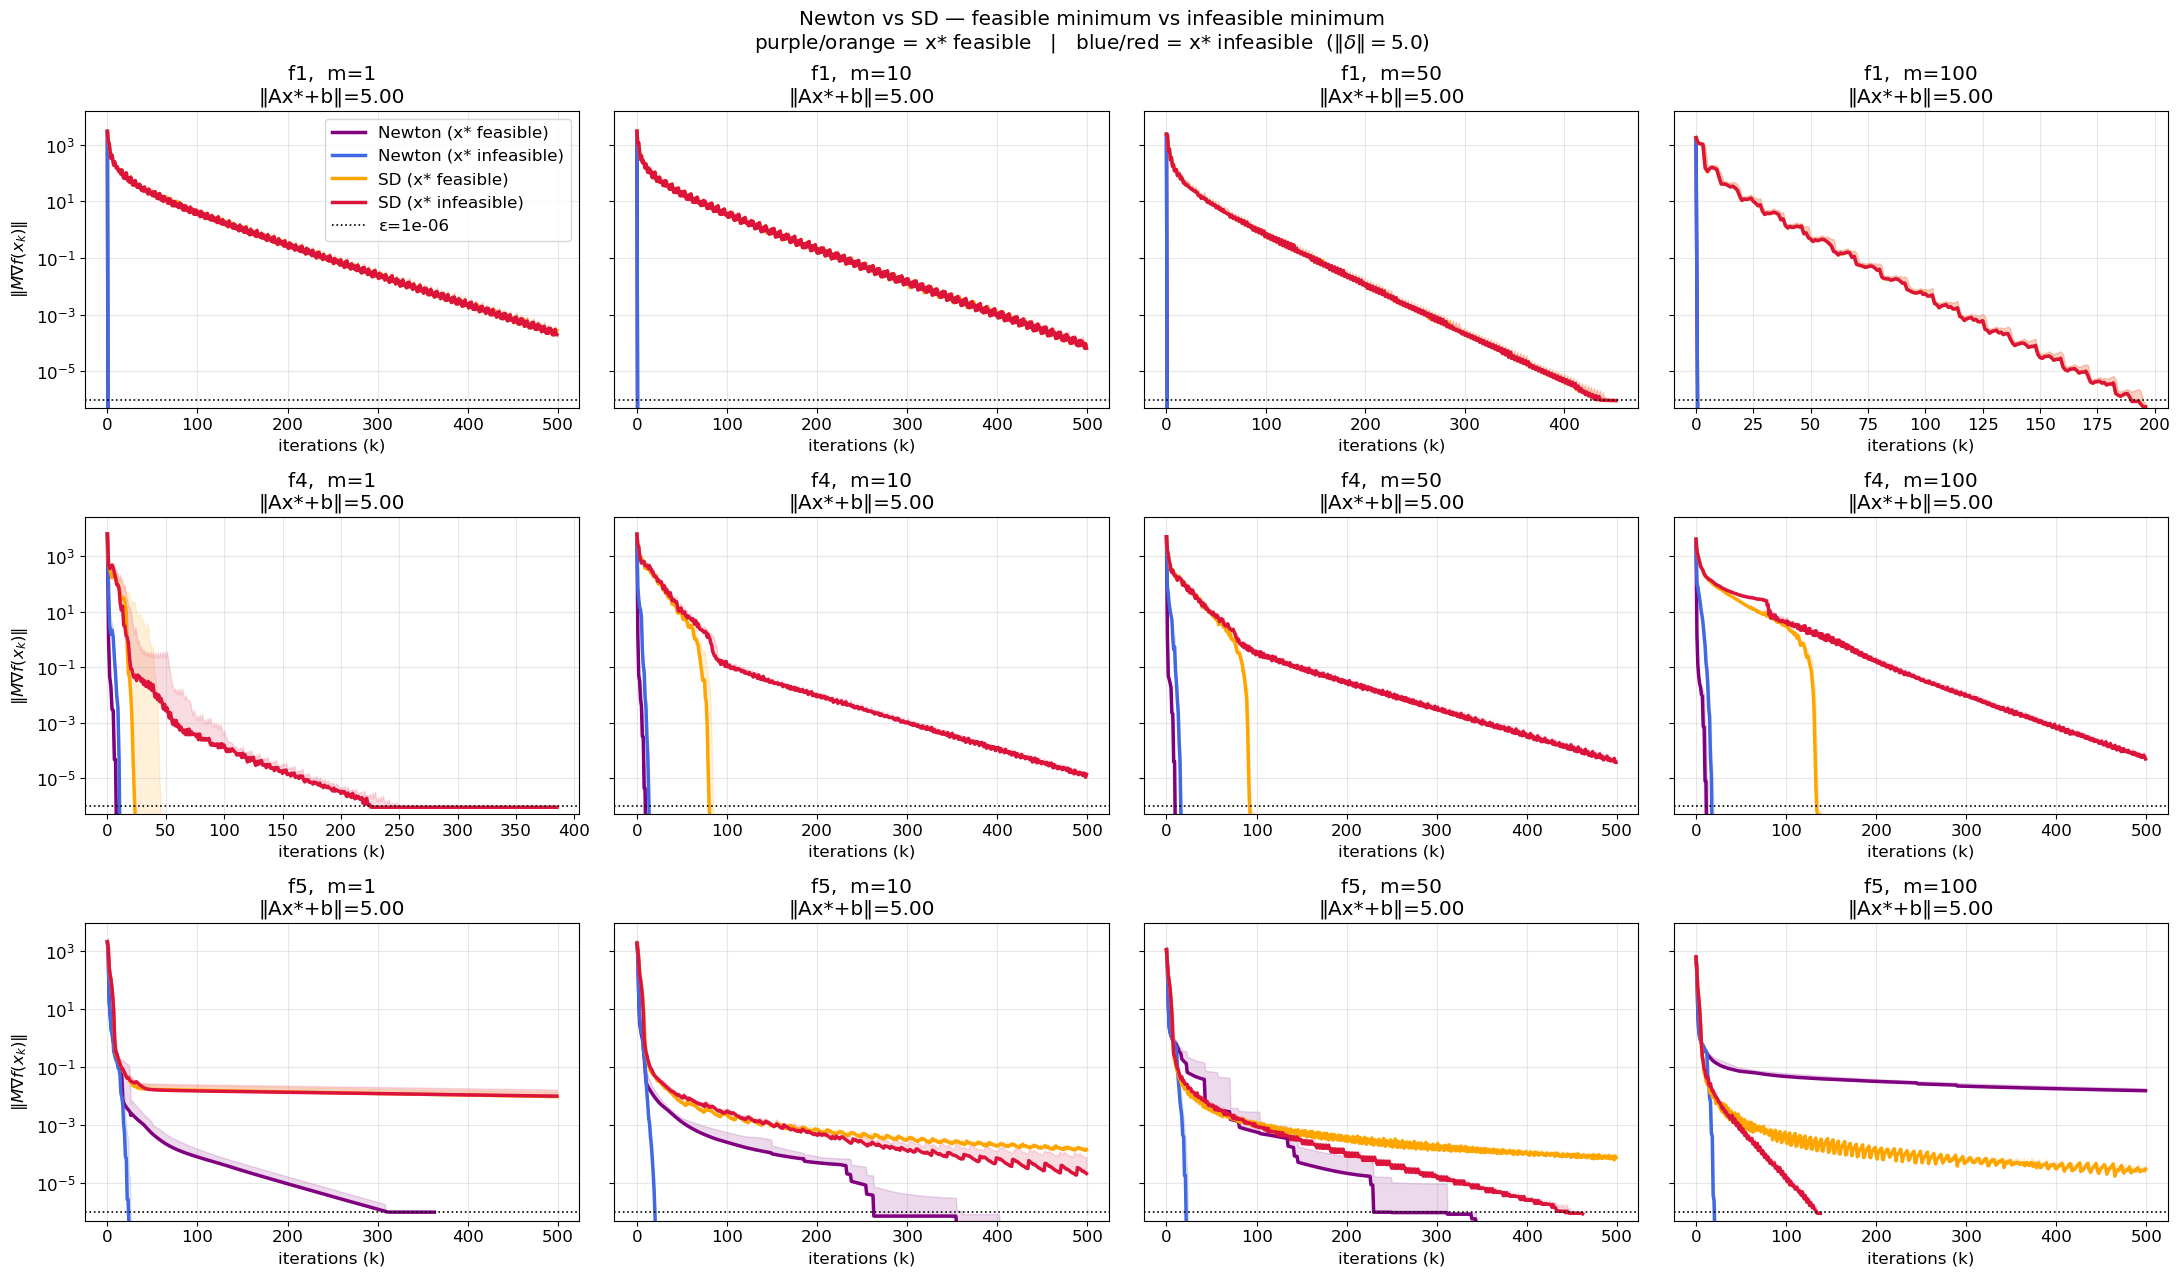
\includegraphics[width=1\linewidth]{newSD.png}
    \caption{Newton vs SD - feasible minimum vs infeasible minimum}
    \label{fig:placeholder}
\end{figure}

Figure 1 is the projected gradient norm $\|M \nabla f(x_k)\|$ vs.\ iterations for constrained Newton's method and steepest descent (SD) applied to $f_1$, $f_4$, and $f_5$ in $\mathbb{R}^{200}$, with $m \in \{1, 10, 50, 100\}$ equality
constraints $Ax + b = 0$. The constraint matrix $A \in \mathbb{R}^{m \times 200}$
is drawn from $\mathcal{N}(0,1)$ and $b = -Ax^*$, so the unconstrained minimum
$x^*$ is feasible. For each $(f, m)$ pair, 10 initial points are generated feasibly by perturbing $x^*$ along $\mathrm{null}(A)$ with variance $\sigma^2 = 10$. Solid lines show the median and shaded bands the 25th--75th percentile over runs, dashed lines show the 99th percentile. Backtracking line search parameters are $\rho = 0.5$, $c_1 = 10^{-4}$. Maximum iterations are 500, and stopping tolerance is$\varepsilon = 10^{-6}$.
\newline
\newline
For \(f_1\), Newton reaches the tolerance in very few iterations in both settings, while Steepest Descent is clearly slower.
The gap between methods grows as \(m\) increases, indicating stronger sensitivity of Steepest Descent to reduced feasible dimension.
For \(f_4\), the infeasible-minimum setup is the most revealing: Newton remains fast, but Steepest Descent develops long linear tails.
This confirms that excluding the unconstrained minimizer mainly hurts first-order methods more than second-order methods.
For \(f_5\), both methods become less uniform, but Newton still attains lower projected-gradient norms in fewer iterations in most cases.
Steepest Descent often plateaus before finally decreasing, especially for larger \(m\), which suggests difficult conditioning on the constraint manifold.
Constraint violations remain near numerical precision, so differences are due to optimization dynamics, not loss of feasibility.
Overall, Newton is the better default method when fast convergence is required under linear equality constraints.
Steepest Descent is simpler and robust, but its runtime cost becomes significant on harder functions and tighter constraint sets.
\newline
\newline
An additional geometric interpretation helps explain the observed trends. 
The feasible set is an affine subspace of dimension $200-m$, and all steps are restricted to its tangent space via the projector $M$. 
As $m$ increases, the dimension of the feasible space decreases, which alters the effective conditioning of the problem within that subspace. 
Steepest Descent is particularly sensitive to this, since it relies purely on first-order information and therefore reacts strongly to anisotropy along the remaining feasible directions. 
Newton’s method, in contrast, incorporates curvature information through the projected Hessian and therefore adapts more effectively to the geometry of the constraint manifold. The infeasible-minimum experiments further illustrate that the constrained solution is not simply a truncated version of the unconstrained trajectory. 
When $x^*$ is infeasible, both methods must move toward the minimiser of $f$ restricted to the affine subspace, which can lie in a direction poorly aligned with the steepest-descent direction. 
This explains the long linear tails observed for Steepest Descent, whereas Newton’s method maintains its characteristic fast local convergence. Finally, the behaviour aligns well with theory: Steepest Descent exhibits linear convergence governed by the condition number of the projected Hessian, while Newton’s method displays locally quadratic convergence once sufficiently close to the constrained minimiser. The numerical results therefore confirm the expected theoretical convergence properties under linear equality constraints.

\section{Conclusion}

We showed that under linear equality constraints, feasible directions lie in the null space of the constraint matrix. 
The numerical experiments confirm theoretical expectations. Newton’s method converges rapidly and remains robust as the number of constraints increases, while Steepest Descent exhibits slower, linear convergence and stronger sensitivity to conditioning. 
Overall, second-order information provides a clear advantage in equality-constrained optimisation.

\end{document}
